
\chapter{Macro-programming}\label{chap:macro-programming}%\mtcaddchapter
\minitoc% Creating an actual minitoc

%% TODO REMEMBER TO DISCUSS THE GRADIENT
Macroprogramming, as a paradigm, 
 has emerged as a pivotal approach in the realm of distributed systems. 
%
It offers a unique perspective, 
 allowing developers to express the \emph{macroscopic behaviour} of a collective system using a singular program.
% 
This chapter delves into the intricacies of macroprogramming, 
 its historical evolution, and its significance in the modern computational landscape, 
 leading to aggregate computing -- a novel macro-programming approach for Cyber-Physical Swarms.

\begin{figure}
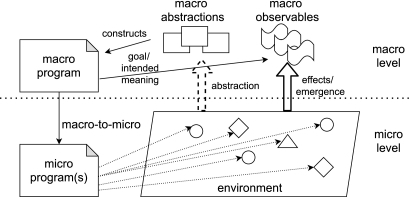
\includegraphics[width=\textwidth]{chapters/img/macro-programming.jpg}
\caption{Overview of macroprogramming}\label{macro:fig:macro-programming}
\end{figure}
\section{The Essence of Macroprogramming}
Macroprogramming  emphasizes the overarching behaviour of a system, abstracting the intricacies of individual components. 
 This abstraction is crucial for systems where the collective behaviour is more significant than the sum of its parts.

The primary motivation behind macroprogramming 
 is to simplify the design and development of complex systems. 
 By providing a higher-level perspective, 
 it allows developers to address system-wide concerns without getting bogged down by the details of individual components. 
 This not only streamlines the development process but also ensures that the system's behaviour is \emph{consistent} and \emph{predictable}.

In essence, macroprogramming is about seeing the \emph{forest} for the \emph{trees}. 
 It recognizes that while individual components (or trees) are essential,
 understanding and managing their collective behaviour (or the forest) is of paramount importance. 
This perspective is particularly relevant in today's interconnected world, 
 where systems often comprise numerous components that need to work in harmony.

Furthermore, macroprogramming leverages macro-level abstractions, 
 such as \emph{collective states}, \emph{groups}, or \emph{spatiotemporal} patterns. 
 These abstractions provide a structured way to think about and design systems, ensuring that they are both \emph{robust} and \emph{adaptable}. 
By focusing on these higher-level abstractions, 
 macroprogramming allows for a more intuitive and efficient approach to system design, 
 making it an indispensable tool in the modern developer's toolkit.
\Cref{macro:fig:macro-programming} provides an overview of the idea behind this paradigm.

Diving deeper into the terminology, 
 terms like ``system programming'', ``centralized programming'', and ``high-level programming'' 
 have been used in various contexts, leading to potential confusion. 
% 
Among these, domain-specific terms like ``global-level programming'', ``swarm programming'', and 
 ``aggregate programming'' stand out. 
%
These terms reflect the diverse perspectives from which macroprogramming can be approached, 
 emphasizing the need for a unified framework that can consolidate these diverse viewpoints. 
%
Such a framework would not only provide clarity but also pave the way for innovative solutions in the realm of systemic behaviour modelling.

\section{Conceptual Framework}

\subsection{Preliminaries}
Macroprogramming addresses the challenge of programming the behaviour of a computational system \( S \), composed of multiple computational entities. Given two entities \( A \) and \( B \) within this system, there are three primary modes to influence their behaviour to promote properties ascribable to \( S \):
\begin{enumerate}
    \item Altering their context, indirectly influencing them. For instance, a change in sensor \( A \) might subsequently affect \( B \).
    \item Interaction, such as triggering their behaviour. If \( A \) is an actuator, its actions might influence \( B \).
    \item Setting their behaviour to produce certain global outcomes when activated.
\end{enumerate}
The term "program" refers to an abstract description executable by a computational entity. Modes (1) and (2) allow an external entity \( C \) to influence \( A \) or \( B \), and consequently \( S \).

\subsection{Macroprogramming: Definition and Basic Concepts}
Macroprogramming is defined as an abstract paradigm for programming the macroscopic behaviour of systems of computational entities. As a paradigm, it's an approach rooted in a mathematical theory or a set of coherent principles. The foundational principles of macroprogramming include:
\begin{itemize}
    \item Micro-macro distinction: Recognizing two primary system levels - macro (global structures) and micro (computational entities).
    \item Macroscopic perspective: Focusing on the system's macroscopic aspects, considering micro-level entities from a global perspective.
    \item Macroprogram: The result of macroprogramming, a program executed by the system adopting the macroscopic perspective.
    \item Macro-to-micro mapping: Implementing how a macroprogram is executed by the system, defining a logic to map macro instructions to micro-level behaviors.
\end{itemize}

\subsubsection{On Micro-Macro and Local-Global Distinction}
The micro-macro distinction is prevalent in various scientific areas, distinguishing smaller elements from larger ones. For programming, a system can be defined based on a boundary condition, distinguishing between the micro and macro dimensions. The goal of macroprogramming is closely tied to the concept of emergence, analysing the relationships between microscopic and macroscopic states.

\subsubsection{On Collectives}
Macroprogramming often targets collectives, groups of similar entities sharing common traits or goals. While heterogeneous collectives exist, they tend to complicate macroprogramming by emphasizing individual perspectives or widening the macro-to-micro gap.

\subsubsection{On Declaratively}
Declarativity is a hallmark of macroprogramming, focusing on the computation's goal rather than its method. This approach abstracts away specific computational aspects, offering high-level abstractions tailored to specific application domains, often resulting in Domain-Specific Languages (DSLs).

\subsection{Historical Evolution and Context}

The historical roots of macroprogramming can be traced back to the pioneering work of Newton and Welsh in 2004. 
 Their research laid the foundation for the application of macroprogramming in the domain of Wireless Sensor Networks (WSNs). 
 These networks, characterized by embedded units equipped with processing, communication, and sensing capabilities, presented unique challenges that necessitated a macroscopic view for effective data processing and logic description. 
The emphasis was on capturing the collective behaviour of these sensor nodes, 
 ensuring efficient data aggregation, processing, and communication.

WSNs were among the first systems that required a departure from traditional programming paradigms. 
 Given the distributed nature of these networks and the limited resources of individual sensor nodes, 
 there was a pressing need to optimize both computation and communication. 
 Macroprogramming emerged as a solution, allowing developers to focus on the overall behaviour of the network rather than the intricacies of individual nodes.

As technology evolved, so did the applications of macroprogramming. 
 The rise of the Internet of Things (IoT) in the subsequent years brought forth a plethora of interconnected devices, each with its own set of capabilities and functions. 
 The complexity of these systems further underscored the importance of a macroscopic approach. Macroprogramming principles were adapted and refined to cater to the diverse requirements of IoT ecosystems.

Furthermore, the emergence of Cyber-Physical Systems (CPSs) and spatial computing introduced new challenges and opportunities for macroprogramming. 
 These systems, which integrate computational processes with physical entities, demanded a holistic approach to ensure seamless interaction and coordination. 
 Macroprogramming, with its emphasis on collective behaviour and high-level abstractions, proved to be an invaluable tool in this context.

Over the years, the principles of macroprogramming have been enriched by interdisciplinary research, drawing insights from fields such as distributed systems, artificial intelligence, and network theory. 
 This confluence of ideas has shaped the evolution of macroprogramming, making it a dynamic and ever-evolving field that continues to adapt to the changing technological landscape.

\section{Aggregate computing}
\subsection{Field-based Computing}
\label{s:background-fieldcomp}

\emph{Field-based computing}~\cite{DBLP:journals/jlap/ViroliBDACP19}
 is an approach
 where computation leverages
 a notion of \emph{computational fields} (\emph{fields} for short)~\cite{DBLP:conf/icra/Warren89,DBLP:journals/pervasive/MameiZL04,DBLP:journals/jlap/ViroliBDACP19}, namely
 distributed data structures evolving in time and associating locations with values.
%
The approach originates from previous work
 like
 Warren's \emph{artificial potential fields}~\cite{DBLP:conf/icra/Warren89}
 and
 \emph{co-fields} from Mamei et al.~\cite{DBLP:journals/pervasive/MameiZL04}.
%
In particular, in co-fields, computational fields represent contextual information, locally sensed by the agents and repeatedly distributed by the agents themselves or the infrastructure according to a propagation rule.
%moreover, they are associated with a propagation rule that determines how they should change as they are distributed.

In this work, by field-based computing we mean a specific programming and computational model,
 also known as \emph{aggregate computing} in literature~\cite{aggregatecomputing},
 which is surveyed in~\cite{DBLP:journals/jlap/ViroliBDACP19}.
% and that we recap in the following.
%%
%In particular, we mean an approach
%  where
In this model,  collective and self-organising behaviour
 is programmed through a composition
 of functions operating on fields
% \emph{computational fields}~\cite{DBLP:journals/jlap/ViroliBDACP19},
% namely distributed data structures, evolving in time,
 mapping a set of individual agents (rather than environment locations)
 to computational values.
%
Therefore, fields can be used to associate a certain domain of agents
 with what they sense, the information they process, and actuation instructions for operating on the environment.
%
Fields are computed locally to the agents
 but are subject to a global viewpoint:
 so, e.g., a field of velocity vectors can be seen as a movement command for an entire swarm, or
 a field of reals can denote what an entire swarm perceives in a certain environment.
%
To understand field-based computing,
 two essential parts have to be considered: the system model
 and the programming model.
 Their interplay is what allows the local actions of the agents
 to yield emergent collective behaviour.

\subsubsection{System Model}
\label{ssec:background:sysmodel}

We consider a network of computing and interacting \emph{agents} situated in some \emph{environment}.

\subparagraph*{Structure.}
%
An \emph{agent} is an autonomous entity
 equipped with \emph{sensors} and \emph{actuators}, which serve as the interface towards a logical or physical \emph{environment}.
%
By a logical point of view\footnote{Actually, such requirements may be relaxed by considering different execution strategies on available infrastructure~\cite{DBLP:journals/fi/CasadeiPPVW20}.}, it also has \emph{state}, a support for \emph{communicating} with other agents, and support for \emph{computing} simple programs.
%
An agent is connected with other \emph{neighbour} agents which collectively form its \emph{neighbourhood}.
%
The set of neighbours depends on a \emph{neighbouring relationship}, which is defined by designers according to the application at hand
and is subject to the constraints exerted by the underlying physical network.
%
A typical neighbouring rule
 is the one that mimics physical connectivity;
 so, e.g., a robot is a neighbour of another robot if it manages to send a message to the latter over the wireless channel.
%
%\meta{FD: @MIRKO is this rule used later in the paper? If no, why we mention it here? RC: @FD this is a useful example to also explain the following rule, which is the one we adopt.}
Another typical neighbouring rule is the one
 based on spatial vicinity;
 so, e.g., a robot is a neighbour of another robot if the infrastructure manages to deliver a message from the former to the latter (e.g., using other robots as relays)
  and these two robots are at an estimated distance smaller than a certain threshold
  (assuming a distance can be estimated through a proper technology).

\subparagraph*{Interaction}
%
Interaction happens by sending messages
 to neighbours, asynchronously.
%
Interaction can also happen in a stigmergic way, by perceiving and acting upon the environment through sensors and actuators.
%
The content of messages and when they are sent and received depend on the agent behaviour.
%
However, in general, as our goal is to model continuous collective behaviours, or self-organising systems,
 we remark that interaction would typically be frequent (in relation to the problem and environment dynamics).

\subparagraph{Behaviour}
%
As per the above consideration,
 the behaviour of any individual agent is best understood
 in terms of repeated enaction of \emph{execution rounds}, where each round consists of the following steps (though some flexibility exists especially in the actuation part):
%
\begin{enumerate}
\item \emph{Context acquisition.} The agent gathers its context by considering its previous state as well as the most recent sensor readings and messages from neighbours.
\item \emph{Computation.} The agent runs a computation against the acquired context, yielding (i) an \emph{output} describing potential actuations; and (ii) a \emph{coordination message} containing all the information to be sent to neighbours for the purpose of coordination at a collective level.
\item \emph{Actuation \rev{and communication}.} The agent performs the actuations described by the program output and dispatches the coordination message to the entire neighbourhood.
\end{enumerate}
%
\rev{
By having every agent repeatedly
 run these sense-compute-act rounds,
 the whole system
 fosters a self-organization process
 whereby
 up-to-date information
 (from the environment and from the agents)
 is continuously incorporated
 and processed,
 typically in a self-stabilising manner~\cite{DBLP:books/mit/Dolev2000}.
}

This system model provides a basic machinery for collective adaptive behaviour, which however requires a proper description of the ``local computation step'': this is fostered by the \emph{field-based programming model} (discussed in \Cref{sec:field-based-programming-model}).
%
\rev{
A \emph{field-based program}
 steers the collective adaptive behaviour of a system,
 which unfolds by having each agent in the system
 evaluate that program
 according to the discussed round-based execution model.
%
Notice that such a program
 specifies both what local processing the agents
 must perform
 and what data they must share with neighbours;
 also, notice that generally the program does not affect the round-based execution protocol---unless advanced forms of scheduling are desired~\cite{lmcs-timefluid}.
%
The distributed execution protocol
 may be provided by a \emph{middleware},
 which will ensure that
 messages are exchanged
 and rounds properly scheduled.
%
The reader can refer to
 \cite{lmcs-timefluid}
 and
 \cite{casadei2022applsci}, respectively,
for a more comprehensive discussion on
 execution and deployment aspects.
}


\subsubsection{Field-based Programming Model}
\label{sec:field-based-programming-model}

Field-based programs can be encoded with field-based programming languages like \scafi{}~\cite{DBLP:conf/isola/CasadeiVAD20}, \rev{which are implementations of \emph{field calculi}~\cite{DBLP:journals/jlap/ViroliBDACP19,scafi-lmcs}, i.e., functional core languages that provide the minimal set of constructs for programming with fields and enable formal analysis}.
%
\scafi{} is a domain-specific language (DSL) embedded in Scala
 which supports field-based constructs
 and offers a library of reusable functions\rev{, some of which are covered in the following}.
%


A field-based expression or program (e.g., programmed in \scafi{}) can be subject
 to a local or global interpretation.
%
Locally, an integer value like \texttt{7} has the usual meaning;
 globally, a \texttt{7} denotes a field where each agent is mapped to a local \texttt{7} (a uniform, constant field).
%
\rev{
For instance, querying a local temperature sensor
 would yield a \emph{field of temperature readings},
 associating space-time events
 (i.e., all the rounds of a network of agents)
 to values denoting the temperatures
 at those locations.
}

Locally, an integer expression \texttt{add(a,b)}, or \texttt{a+b}, has the usual meaning, given by the sum of \texttt{a} with \texttt{b};
 globally, it denotes the application of a field of functions \texttt{add}, or \texttt{+},
 on a field \texttt{a} and a field \texttt{b},
 yielding a field given by the sum of \texttt{a} and \texttt{b}
 in an agent-wise fashion (notice that \texttt{a} may be a non-uniform non-constant field having different local values for different agents over time).

The programming model does not deal directly with global fields (which are essentially a denotational construct),
 but it deals only with \emph{neighbouring fields},
 which enable one agent to collect data from its neighbours.

\rev{
Generally, field calculi feature constructs to
 (i) evolve values across time, by transforming a value computed at a previous round into a new value;
 (ii) exchange data with neighbours, where received data is reified by neighbouring fields;
 (iii) conditionally break a computation into parts,
 defining distinct domains of collective computation.
}
%
\rev{However,} in the following, we \rev{only} briefly present a subset of the field-based computing building blocks used for sensing-based clustering\rev{, as the details of field calculi are not required to understand the contribution of this manuscript}.
%
See~\cite{DBLP:journals/jlap/ViroliBDACP19} for more details on how these blocks are actually developed.

Typically, in field-based computing applications, we are dealing with sharing and collecting information from/to a device.

To do this, the \lstinline|gradient| is an essential construct~\cite{DBLP:conf/saso/AudritoCDV17}.
%
This block produces a numeric field that expresses the minimum distance from a source zone following a certain metric (e.g., Euclidean distance).
%
Hence, it maps a Boolean field (\lstinline|true| where a node is a source, \lstinline|false| otherwise) into a distance field from the closest source. The signature of the function is defined as\footnote{\rev{In Scala, keyword \lstinline|def| introduces a named function; after the name, it follows a list of parameters of the form \lstinline|name:Type|; after the parameter list, the return type of the function is specified.}}:
%
\begin{lstlisting}
def gradient(source: Boolean, metric: Metric): Double
\end{lstlisting}
%
\rev{This function is resilient to changes in the source field and metric field, self-stabilising to the correct field of minimum distances to the closest source once input fields stabilize.}
%
\rev{Gradients support \emph{information flows}, which are fundamental constructs for designing self-organising systems~\cite{DBLP:conf/saso/WolfH07}.}
%
\rev{Indeed, t}hrough this construct, it is possible to share generic data (a position, a temperature, etc.) towards this resulting distance field.
%
Such propagation of data from a source of a gradient outwards
 is captured by a
\lstinline|broadcast| function \rev{(generic in type parameter \lstinline|D)|}:
\begin{lstlisting}
def broadcast[D](source: Boolean, data: D): D
\end{lstlisting}
%
%The information in these two previous operators flow from the source nodes to the others nodes.
When we want to aggregate data in source agents, we use the block \lstinline|C| (collect) instead~\cite{audrito2021jcee-distributed-collection}:
\begin{lstlisting}
def C[V](p: Double, acc: (V, V) => V, local: V, null: V): V
\end{lstlisting}
%
In this signature, \lstinline|p| is a potential field usually computed through \lstinline|gradient|; \lstinline|acc| is the logic that combines \rev{locally perceived data with that received from neighbours}; \lstinline|local| is the local data we want to collect at a point in space (e.g. a position); and \lstinline|null| is the null data for the \lstinline|acc| operation (e.g. if we collect a real value, the \lstinline|null| value could be 0).
%
This is also an essential operation for the definition of collective behaviours: it enables, e.g. computation of the average temperature in a certain zone covered by agents.

\rev{
As an example, consider a network of agents
 where a sparse set of leaders have been elected.
%
Suppose that we want to break the system
 into several regions, each one ruled by one leader,
 and that we want every agent
 to know how many members are in their region.
%
This can be coded as follows:
}
\begin{lstlisting}
val leader: Boolean = // true on leader devices
val potential: Double = gradient(leader, metric())
val collect: Int = C[Int](potential, (sum,v)=>sum+v, 1, 0)
val count: Int = broadcast[Int](leader, collect)
\end{lstlisting}
\rev{
A region is indirectly defined by the corresponding leader; each agent has to simply descend the gradient to locate its leader (and hence its region).
%
Along the \lstinline|potential| towards leaders,
 a contribution of \lstinline|1| is accumulated
 for each agent.
%
To propagate the complete count on the whole region, it is then sufficient to \lstinline|broadcast| the \lstinline|leader|'s \lstinline|collect| value outwards.
}

Future work could be devised in multiple directions.
%
First, it could be interesting to stress and possibly refine
the algorithm on more extreme environmental conditions,
 or to investigate it under different assumptions (e.g., a more constrained or rich system model).
%
Secondly, it could be interesting to compare (or combine) the meta-algorithm against (with)
 automated swarm behaviour design methods
 like multi-agent reinforcement learning.
%
Last but not least, we would like to evaluate our algorithms on real use cases, e.g. in smart logistics and precision agriculture scenarios, by implementing them %using the FCPP field-based computing language and deploying them
on actual drones or robots.
\subsection{ScaFi}\label{sec:scafi}
%!TeX root = thesis-main.tex
 \emph{\scafi{} (Scala-Fields)} is
 an aggregate programming toolkit
 that comprises an internal DSL (language and virtual machine)
 as well as supporting components for the simulation
 and execution %deployment 
 of aggregate systems.

\subparagraph{Software description}
\label{}
\scafi{} is a multi-module Scala project hosted on GitHub\footnote{\url{https://github.com/scafi/scafi}}.
%
It provides DSL and API modules for 
 writing, testing, and running aggregate programs, namely programs expressed according to the aggregate programming paradigm~\cite{aggregatecomputing,DBLP:journals/jlap/ViroliBDACP19}.
%
\subparagraph{Software Architecture}
\label{sec:scafi-arch-design}

The high-level architecture of \scafi{} is depicted in \Cref{fig:scafi-arch}.
It consists of the following main components: %(where each component is an SBT module and deployable artifact):
\begin{itemize}
\item \texttt{scafi-commons} | provides basic abstractions and utilities (e.g., spatial and temporal abstractions);
\item \texttt{scafi-core} | provides an aggregate programming DSL (syntax, semantics, and a virtual machine for evaluation of programs), together with a ``standard library'' of reusable functions;
\item \texttt{scafi-stdlib-ext} | provides extra library functionality that requires external dependencies and is hence kept separated from the minimalist \texttt{scafi-core};
\item \texttt{scafi-simulator}: provides basic support for simulating aggregate systems;
\item \texttt{scafi-simulator-gui} | provides a GUI for visualizing and interacting with simulations of aggregate systems;
\item \texttt{spala} (``spatial Scala''---i.e., a general aggregate computing platform\footnote{aggregate computing is rooted in spatial computing~\cite{DBLP:journals/corr/abs-1202-5509}.}) | provides an actor-based aggregate computing middleware
(independent of the \scafi{} DSL and potentially applicable to other aggregate programming languages as well)
based on the Akka toolkit~\cite{akka};
\item \texttt{scafi-distributed} | ScaFi integration-layer for \texttt{spala},
which can be leveraged to set up actor-based deployments of \scafi{}-programmed systems.
\end{itemize}
 
\begin{figure}
\centering
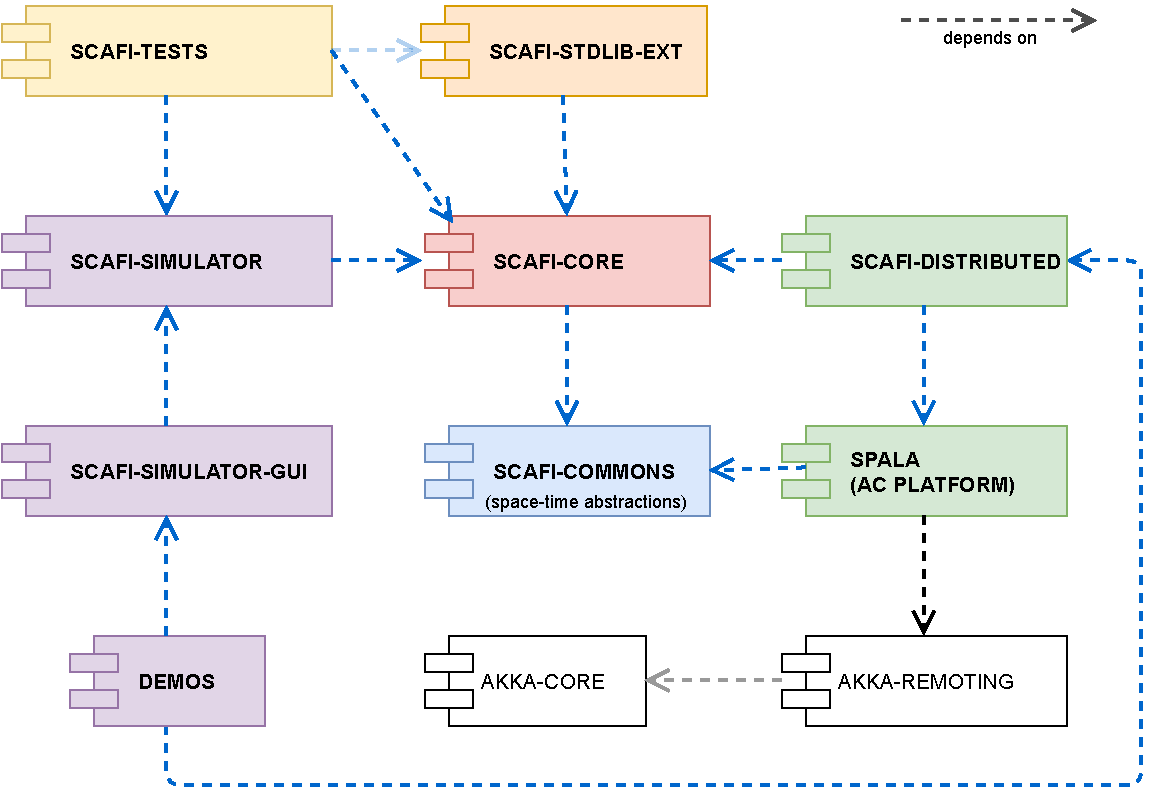
\includegraphics[width=0.8\textwidth]{papers/softwarex2021/imgs/scafi-project-org.pdf}
\caption{High-level architecture of the \scafi{} toolkit.}
\label{fig:scafi-arch}
\end{figure}

\begin{figure}
\centering
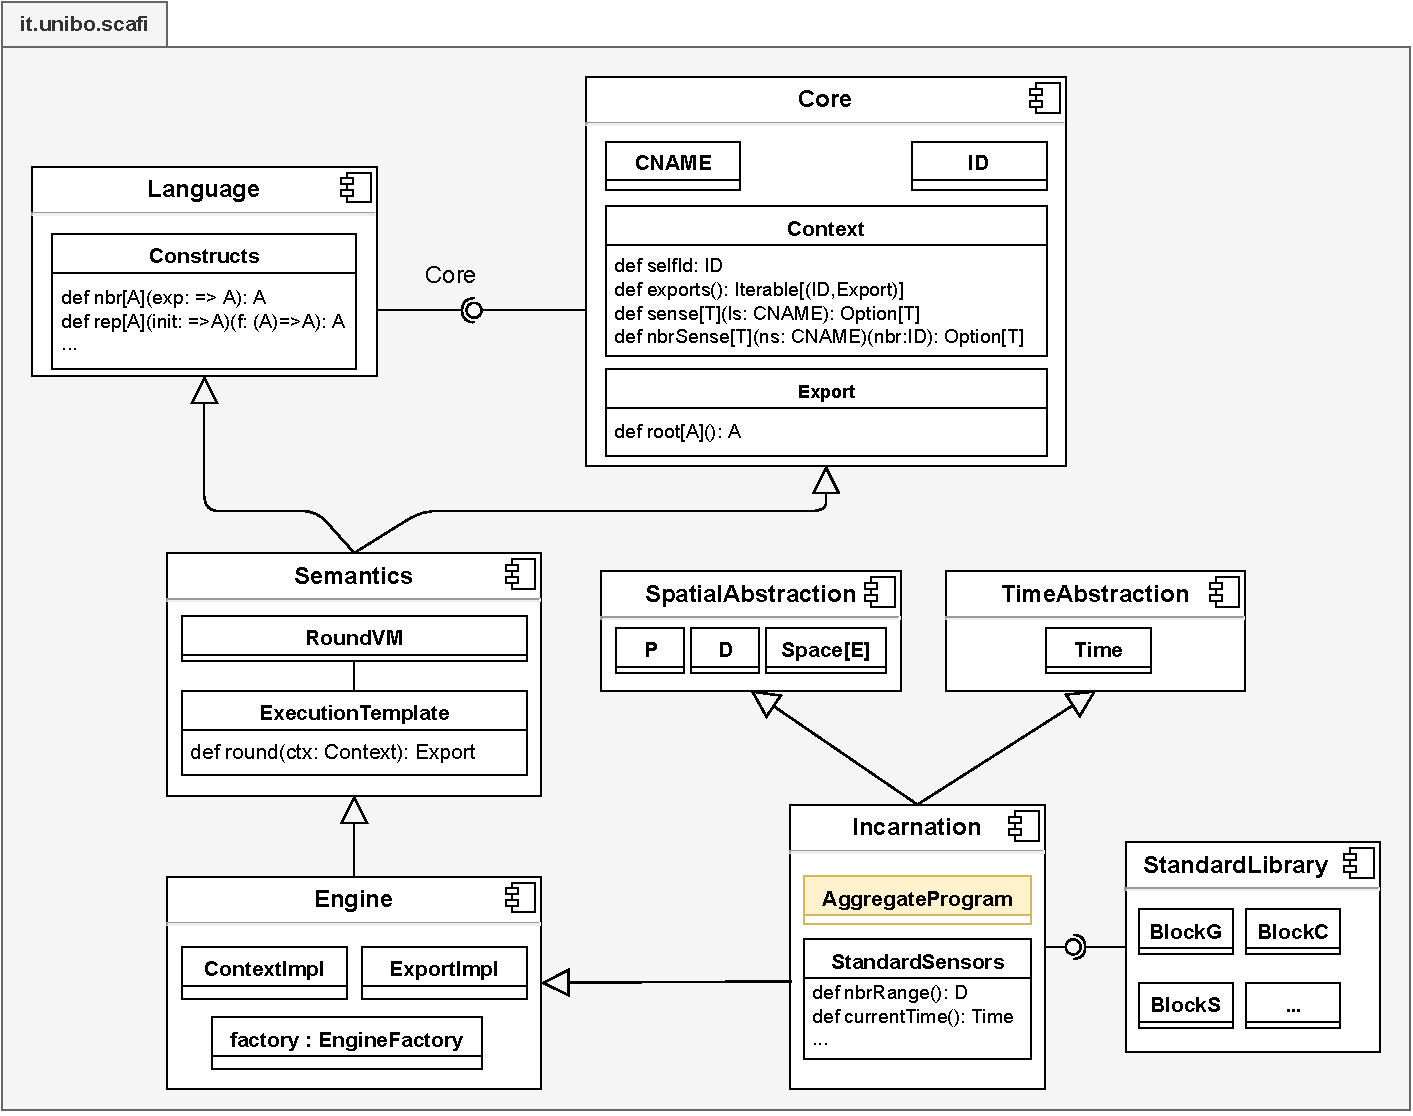
\includegraphics[width=0.8\textwidth]{papers/softwarex2021/imgs/scafi-design.drawio.pdf}
\caption{\revision{Design of the core of \scafi{} (DSL).}}
\label{fig:scafi-design}
\end{figure}

\revision{
\scafi{} leverages the concept of an \emph{incarnation},
 namely a concrete ``family of types''~\cite{DBLP:conf/oopsla/OderskyZ05} 
 that is progressively refined through inheritance, composed, and finally instantiated into an object (cf. the Scala \emph{cake pattern}~\cite{Hunt2013cakepattern,DBLP:conf/oopsla/OderskyZ05})
 which ultimately provides access 
 to a type-coherent set of features.

\Cref{fig:scafi-design} provides an excerpt 
 of the main Scala traits 
 with some types and objects they define.
%
Trait \texttt{Core} provides the abstract fundamental types: \texttt{CNAME} for capability names,
\texttt{ID} for device identifiers,
\texttt{Context} for the input environment of computation rounds,
and \texttt{Export} for the outcomes of computation rounds.
%
Trait \texttt{Language} 
 provides the syntax of the DSL in terms of methods, through interface \texttt{Constructs}.
%
Trait \texttt{Semantics} and \texttt{Engine}
 implement the DSL construct semantics,
 providing a template for \texttt{AggregateProgram} base class defined in the \texttt{Incarnation} trait. 
The incarnation also exposes \texttt{StandardSensors} in terms of, e.g., \texttt{SpatialAbstraction}'s and \texttt{TimeAbstraction}'s types for positions (\texttt{P}), distances (\texttt{P}), and time.
%
The \texttt{StandardLibrary} is provided by leveraging 
 what an incarnation provides,
 providing traits of functionality to be mixed into \texttt{AggregateProgram}s.
}

\paragraph*{Software Functionalities}
\label{}

\subparagraph*{Expressing aggregate programs through a Scala DSL}
\label{sec:express-programs}
%
Module \texttt{scafi-core}
 exposes,
 through incarnations,
 an \texttt{AggregateProgram} trait
  that provides access to 
  aggregate programming constructs---following 
  a variant of the field calculus~\cite{DBLP:journals/tocl/AudritoVDPB19,DBLP:journals/jlap/ViroliBDACP19}
  formalized in~\cite{DBLP:conf/isola/CasadeiVAD20}.
%
This single program defines -- from a global perspective -- 
 the collective adaptive behaviour 
 of an entire %system or 
 ensemble of computational devices.
%
Besides the core constructs,
 this module also provides ``standard library'' traits
 providing access to reusable functions of aggregate functionality.
%
For instance, by mixing trait \texttt{Gradients}
 into an \texttt{AggregateProgram} subclass,
 a developer gets access to \emph{gradient functions}~\revision{\cite{DBLP:conf/sac/BealBVT08,DBLP:journals/tomacs/ViroliABDP18}}, used to 
 continuously compute (over space and time) the self-healing field of minimum distances of each node from a set of source nodes. %---possibly in mobile and faulty environments.
%
Several such traits are available
 to provide other key building blocks
 for self-organising applications~\revision{\cite{DBLP:conf/saso/WolfH07,DBLP:journals/tomacs/ViroliABDP18}} (e.g., \texttt{BlockG} \revision{for gradient-wise information propagation}, \texttt{BlockC} \revision{for gradient-wise information collection}, \texttt{BlockS} \revision{for sparse choice or leader election})
 or experimental language features
 (e.g., the \texttt{spawn} function for concurrent aggregate processes~\revision{\cite{DBLP:journals/eaai/CasadeiVAPD21,testa2022processes}}\revision{, for modelling independent and overlapping aggregate computations}).
%
\subparagraph*{Virtual machine for the local execution of aggregate programs}
%
An \texttt{AggregateProgram} instance 
 is a function
 mapping a \texttt{Context}
 (the set of inputs needed by an individual device
  to properly evaluate the program locally)
 to an \texttt{Export}
 (the tree of values that has to be shared 
  with neighbours to effectively coordinate and promote 
  the emergence of collective behaviours).
%
Using this API,
 a developer can 
 integrate ``aggregate functionality''
 into its system---what remains to be specified are the
 details of the aggregate execution model and the communication among devices,
 that may change in different applications.
%
Devices must continuously run the aggregate program,
but the scheduling of these computation rounds can be tuned
as the application needs~\cite{DBLP:journals/lmcs/PianiniCVMZ21}.
%
\texttt{Export}s must be shared with neighbouring devices to allow them
to properly set up their \texttt{Context}s,
but the network protocol to be used to do so can be selected
independently of the program.
 
\subparagraph*{Simulation support}
%
In order to simulate an ``aggregate system'',
 it is necessary to: 
\begin{enumerate}
  \item define the set of computational devices that make up the aggregate, including their sensors and actuators;
  \item define the aggregate topology, i.e., 
  some application-specific \emph{neighbouring relationship}
  from which the set of \emph{neighbours}
  of each device can be determined;
  \item define the aggregate program to be executed;
  \item define a certain dynamics of the system
  by proper scheduling of computation rounds,
  and the environment
  by proper scheduling of changes in sensor values.
\end{enumerate}

%
Module \texttt{scafi-simulator}
 provides this basic support.
%
It exposes some factory methods
to configure simulations properly
 (e.g., it supports ad-hoc and spatial distance-based connectivity rules)
 and an API to run and interact with simulations.
%
Then, module \texttt{scafi-simulator-gui}
 provides a convenient graphical user interface
 to launch and visually show simulations in execution.
%
We remark that these modules currently support basic simulation scenarios
 and are mainly meant for quick experiments
 or as a starting basis for ad-hoc simulation frameworks.
 
\subparagraph*{Experimental or work-in-progress features: actor-based middleware}
%
Regarding the construction of actual systems, 
 \scafi{}
 provides
 an actor-based implementation
 of the aggregate execution model~\cite{DBLP:series/lncs/CasadeiV18},
 in the \texttt{spala} (\texttt{Spa}tial Sca\texttt{la}) module,
 which is instrumental for integrating aggregate computing
 into existing systems and distributed architectures~\cite{DBLP:series/lncs/CasadeiV18}.
%
Indeed, aggregate computing systems
 can be designed, deployed, and executed 
 according to different
 architectural styles 
 and concrete architectures~\cite{DBLP:journals/fi/CasadeiPPVW20}.
%
So, \scafi{} provides \emph{two} main implementations of the middleware,
 in package \texttt{it.unibo.scafi.distrib.actor},
 for purely peer-to-peer 
 (sub-package \texttt{p2p})
 and server-based designs
 (sub-package \texttt{server}).
%
The main abstraction
 is the \texttt{DeviceActor},
 which exposes a message-based interface
 for controlling and interacting with
 an individual logical node of the aggregate system.
%
Then, an object-oriented façade API is provided to set up a system of middleware-level actors. 

%\subparagraph{Sample code snippets analysis (optional)}
%\label{}

%\subparagraph{Illustrative Examples}
\paragraph*{Features}
\label{s:impact}
\scafi{}
 has been used 
 in aggregate computing-related research~\cite{DBLP:journals/eaai/CasadeiVAPD21,audrito2022ecoop-xc,DBLP:conf/coordination/AguzziCV22,
 DBLP:conf/fmec/CasadeiV19,DBLP:conf/IEEEscc/CasadeiTVD19,DBLP:journals/scp/CasadeiAV18,DBLP:journals/jsan/CasadeiAV21,DBLP:conf/coordination/CasadeiVRA21,casadei2022applsci,arxiv2020scafi-nc},
  touching themes such as 
  software engineering, 
  computational models, and
  distributed systems/algorithms.
%
The impact of \scafi{}
 can be understood in terms of 
 existing and prospective contributions, 
 discussed in the following.

\subparagraph*{Interplay between programming language design and foundational research} 
%
The implementation of the \scafi{} DSL
 has inspired a variant of the field calculus
 which arguably supports easier embeddability
 into mainstream programming languages~\cite{DBLP:conf/isola/CasadeiVAD20,arxiv2020scafi-nc}.

\subparagraph*{High-level programming models}
%
The previous discussion  
 makes the case for ``DSL stacking''~\cite{DBLP:conf/icsoft/HummE10}.
%
Indeed, by leveraging the aforementioned aggregate process extension, 
 it is possible to reduce the abstraction gap
 needed to implement \emph{situated tuples}~\cite{DBLP:conf/coordination/CasadeiVRA21}\revision{,
 which is a Linda-like model~\cite{DBLP:journals/toplas/Gelernter85} for coordinating processes where tuples and tuple operations are situated in space}.
%
By mapping high-level specifications into aggregate programs, it is sometimes straightforward to develop resilient distributed implementations---as in~\cite{DBLP:journals/jss/AudritoCDSV21},
 where translation rules from 
 spatial logic formulas
 to field calculus expressions
 enable seamless construction of decentralized monitors for such formulas.

\subparagraph*{Web-friendliness}
%
By leveraging Scala.js~\cite{DBLP:conf/scala/Doeraene18}, \scafi{} can be easily 
 accessed through JavaScript,
 which promotes cross-platform language design 
 and reuse of functionality in the browser
 (to support web applications without the need of server-side components).
%
This paved the path 
 to \scafiweb{}~\cite{DBLP:conf/coordination/AguzziCMPV21},
 a web playground for aggregate programming.
%

\subsection{Alchemist}\label{coordination2023:alchemist}

Alchemist\footnote{\url{http://alchemistsimulator.github.io/}}~\cite{DBLP:journals/jos/PianiniMV13} is meta-simulator
 mainly designed for simulating complex distributed systems 
 in a rich variety of scenarios like swarm robotics~\cite{Casadei2021},
 large-scale sensor networks~\cite{Aguzzi_2022}, crowd simulation~\cite{Beal2015},
 path planning, and even morphogenesis of multi-cellular systems.

The simulator is \emph{meta} in nature, 
 as it is based on general abstractions 
 that can be mapped to specific use cases (i.e., \emph{incarnations}).
% 
Inspired by biochemistry, 
 the meta-model consists of a set of \emph{nodes} 
 that exist in an \emph{environment} and are linked together by \emph{relationship} rules. 
 Each node contains a sequence of \emph{molecules} and \emph{reactions}. 
%
 A \emph{molecule} represents a variable, 
 which acts as a container for data. 
 \emph{Reactions} instead are events that occur based 
 on a set of \emph{conditions}, 
 and are fired according to a time distribution, 
 producing an effect that is described as an action. 
This abstraction allows the simulator to be flexible 
 and adaptable to a variety of use cases and node numbers 
 (it could support thousands of nodes), 
 while maintaining a consistent underlying structure.

 The Alchemist simulator features four incarnations: 
  biochemistry, sapere, protelis, and \scafi{}, 
  each with a different way of modeling molecules and actions. 
The sapere incarnation uses a set of ground Linda-like tuples 
 to model concentration and has been used for crowd evacuation and resource discovery simulations. 
The protelis incarnation defines concentration as a Java Object and is commonly used in the literature for various simulations, 
 including crowd tracking and drone coordination. 
The \scafi{} incarnation supports the \scafi{} Scala DSL 
 and has been used in distributed peer-to-peer chats and situated problem-solving.

Alchemist offers an effortless method for loading simulations. 
 The process requires a YAML file that includes essential parameters, 
 such as the incarnation type, neighbour connection model, and node deployment. 
 In \Cref{coordination2023:fig:alchemist}, we have provided an example YAML file 
 that creates a simulation using the \scafi{} incarnation (first row). 
 It also defines the neighbourhood relationship based on fixed distances (0.5 in this case), 
 placing nodes in a fixed grid of size 10x10 starting at -(5,5) and ending at (5,5), 
 with a node-to-node distance of 0.25. 
 Finally, it loads the \scafi{} program called ``program'', 
 which is evaluated at each node with a frequency of 1. 
\begin{figure*}
\centering
\begin{subfigure}[b]{0.49\textwidth}
    \centering
    %% change the listing size to small with the correct font family
    \begin{lstlisting}[language=yaml, basicstyle=\small\ttfamily, caption={An Alchemist simulation example.}, captionpos=b, label=coordination2023:fig:alchemist-yaml]
incarnation: scafi
network-model:
    type: ConnectWithinDistance
    parameters: [0.5]
deployments:
    type: Grid
    parameters: [-5,-5,5,5,0.25,0.25]
    /*dynamics of the simulation*/
    programs: 
        - program:
        - time-distribution: 1
            type: Event
            actions: 
            - type: RunScafiProgram
              parameters: [program]
        - program: send
\end{lstlisting}
\end{subfigure}
\hfill
\begin{subfigure}[b]{0.49\textwidth}
    \centering
    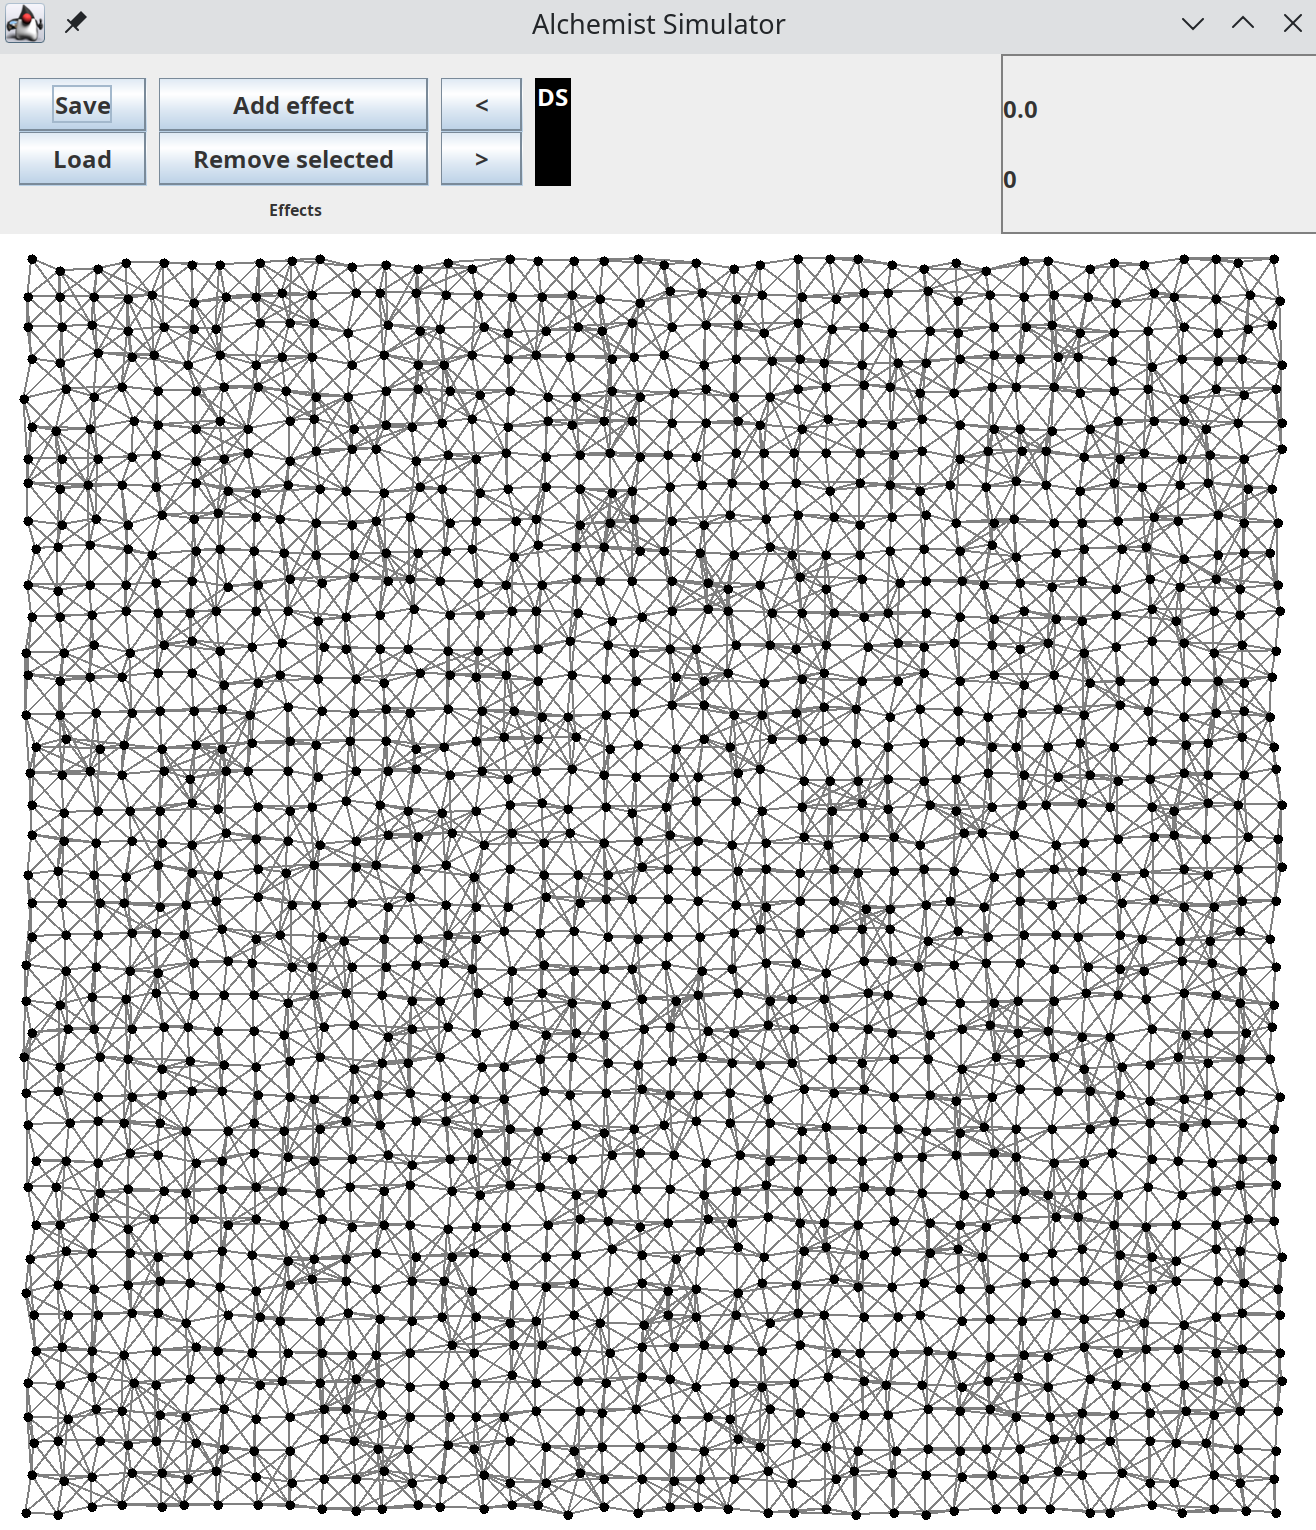
\includegraphics[width=\textwidth]{papers/coordination2023/imgs/alchemist.png}
\end{subfigure}
\caption[An Alchemist simulation example]{An Alchemist simulation example. 
    The simulation result on the right is obtained 
    by running the simulation described on the left.
    }
\label{coordination2023:fig:alchemist}
\end{figure*}

\section{Final Remarks}

Macroprogramming, with its focus on the macroscopic behaviour of systems, 
 has proven to be an invaluable tool in the computational world. 
%
From its early applications in WSNs to its modern-day relevance in IoT and CPSs, 
 it has consistently demonstrated its utility. 
As we move towards an increasingly interconnected world, 
 the principles of macroprogramming will undoubtedly play a pivotal role in shaping the future of computational systems.


%\printbibliography